\documentclass[10pt, a4paper]{article}
\usepackage[paper=a4paper, left=1.5cm, right=1.5cm, bottom=1.5cm, top=3.5cm]{geometry}
\usepackage[utf8]{inputenc}
\usepackage[T1]{fontenc}
\usepackage[spanish]{babel}
\usepackage{indentfirst}
\usepackage{fancyhdr}
\usepackage{latexsym}
\usepackage{lastpage}
\usepackage{calc}
\usepackage{caratula}
\usepackage{fancyhdr}
\usepackage{graphicx}


\titulo{Trabajo Práctico 2\\SIMD}
\fecha{02 / 10 / 2012}
\materia{Organización del Computador II}
\grupo{Grupo KM 20}
\integrante{Fuentes Bahamondes, Gonzalo Guillermo}{412/10}{ness00@gmail.com}
\integrante{Marquez, Matías}{703/08}{sir.incognita@gmail.com}
\integrante{Vanotti, Marco}{229/10}{mvanotti@dc.uba.ar}

\def\contentsname{Índice}

\begin{document} 

    \maketitle

    \tableofcontents

    \pagestyle{fancy}
    \lhead{Fuentes Bahamondes, Marquez, Vanotti}
    \rhead{Orga 2 - SIMD}

    \newpage

    \section{Introducción}

    \section{Desarrollo}
    
                \subsection{Monocromatizar Uno}
            \subsubsection{Implementación ANSI-C (SISD)}
                En esta implementacion se itera fila por fila, píxel por píxel, computando un píxel por iteración usando aritmética de enteros provista por C. El algoritmo es el mostrado por los docentes. Se obtienen los bytes de los correspondientes valores RGB, y se satura el resultado de la operacion (R + 2G + B) / 4 
            \subsubsection{Implementación ASSEMBLER (SIMD)}
                En nuestra implementación, calculamos de a 6 pixeles por iteracion. Para lograr esto, cargamos en los registros xmm0, xmm1, xmm2 y xmm3, las direcciones de forma tal que en el primer byte de cada registro, queden los valores B G G R de cada pixel respectivamente. Luego usamos la instrucción PSHUFB para reorganizar los registros como se ve en la imagen.
                
                \begin{figure}[htb]
                \begin{center}
                \leavevmode
                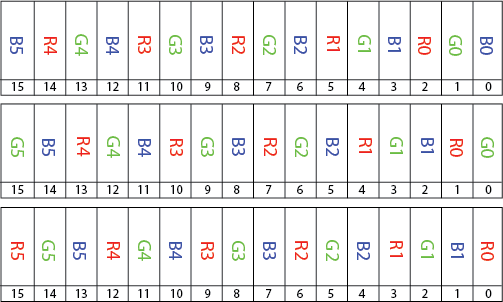
\includegraphics[width=0.5\textwidth]{carga_bytes_rgb.png}
                \end{center}
                \caption{Carga de bytes BGR}
                \end{figure}
                
                \begin{figure}[htb]
                \begin{center}
                \leavevmode
                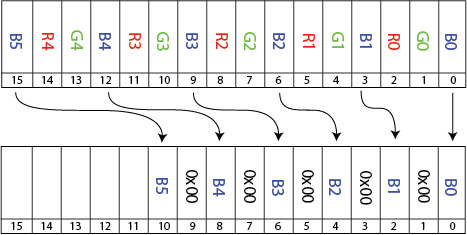
\includegraphics[width=0.5\textwidth]{gris_epsilon_uno_pshub.png}
                \end{center}
                \caption{pshufb para extender a dword}
                \end{figure}
                
                Luego de eso, nos quedan los registros con 6 words sin signo. Los sumamos, shifteamos usando la operación psraw 2 bits a la derecha cada word para dividir por 4. Hacemos un pack para pasar de words a bytes unsigned saturados. En xmm0 nos quedan los primeros 6 bytes con los valores de los píxeles finales. \newpage
                
                \begin{figure}[htb]
                \begin{center}
                \leavevmode
                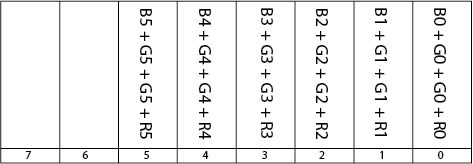
\includegraphics[width=0.5\textwidth]{gris_epsilon_uno_suma.png}
                \end{center}
                \caption{se suman los distintos colores}
                \end{figure}
                
                \begin{figure}[htb]
                \begin{center}
                \leavevmode
                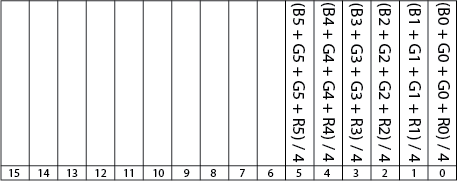
\includegraphics[width=0.5\textwidth]{gris_epsilon_uno_pack.png}
                \end{center}
                \caption{se transforman los resultados a bytes saturando}
                \end{figure}
                
                Finalmente, movemos los 64 bits más bajos de xmm0 a rax, y de ahí a memoria. Como solo tenemos 6 bytes en RAX que sirven, movemos EAX a memoria, shifteamos 32 bits a la derecha y movemos AX a memoria. Luego se pasa a la siguiente iteración.

        \subsubsection{Comparación de Performance (SISD vs SIMD)}

Acá va la comparación de performance entre C y ASM
 \newpage
                \subsection{Monocromatizar Infinito}
            \subsubsection{Implementación ANSI-C (SISD)}
                Esta implementación es análoga a la de Monocromatizar Uno, solo que en vez de storear el resultado de una operación, calculamos el máximo de los 3 valores RGB correspondientes. Se procesa de un píxel a la vez. 
            \subsubsection{Implementación ASSEMBLER (SIMD)}
                El método para cargar las cosas en memoria es similar al de Gris Epsilon Uno también. Solo que el valor G se carga una sola vez (Es decir, en el primer byte de XMM0 queda B, en el primer byte de XMM1 queda G y en el primer byte de XMM2 queda R). Luego usando la instrucción PMAXUB obtenemos el valor máximo de cada byte entre esos registros y los dejamos en XMM0, como se ve en las imágenes.
                
                \begin{figure}[htb]
                \begin{center}
                \leavevmode
                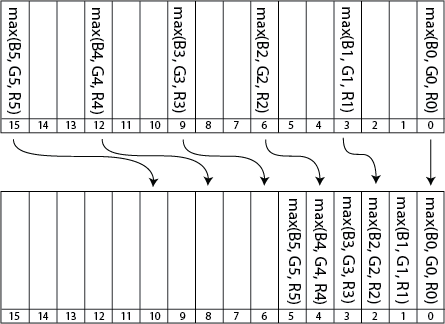
\includegraphics[width=0.5\textwidth]{gris_epsilon_infinito_pshub.png}
                \end{center}
                \caption{pshufb para acomodar los resultados}
                \end{figure}
                
                Luego, hacemos un PSHUFB para poder ordenar los valores de una forma que nos resulte cómoda para pasarlos a memoria, borrando los datos que no nos sirven. No hay problema al usar PSHUFB porque al no haber ni sumas ni restas no tenemos que saturar nada. El método para copiar a memoria es igual al de Monocromatizar Uno.

        \subsubsection{Comparación de Performance (SISD v SIMD)}

Acá va la comparación de performance entre C y ASM
 \newpage
            \subsection{Combinar}
        \subsubsection{Implementación ANSI-C (SISD)}
        \subsubsection{Implementación ASSEMBLER (SIMD)}
        \subsubsection{Comparación de Performance (SISD vs SIMD)}
 \newpage
            \subsection{Normalizar Local}
        \subsubsection{Implementación ANSI-C (SISD)}
        \subsubsection{Implementación ASSEMBLER (SIMD)}
        \subsubsection{Comparación de Performance (SISD vs SIMD)}
 \newpage
            \subsection{Pixelar}
        \subsubsection{Implementación ANSI-C (SISD)}
        \subsubsection{Implementación ASSEMBLER (SIMD)}
        \subsubsection{Comparación de Performance (SISD vs SIMD)}
 \newpage
            \subsection{Recortar}
        \subsubsection{Implementación ANSI-C (SISD)}
        \subsubsection{Implementación ASSEMBLER (SIMD)}
        \subsubsection{Comparación de Performance (SISD vs SIMD)}
 \newpage
            \subsection{Ondas}
        \subsubsection{Implementación ANSI-C (SISD)}
        \subsubsection{Implementación ASSEMBLER (SIMD)}
        \subsubsection{Comparación de Performance (SISD vs SIMD)}
 \newpage


    \section{Conclusión}
    
        A pesar de la mayor dificultad para implementar y pensar como trabajar con vectores utilizando SIMD, la diferencia de performance no es para nada despreciable por lo que vale la pena para este tipo de aplicaciones, donde se realiza numerosas veces la misma aritmética.
        
\end{document}

